\section{Error Analysis}\label{error-analysis}

\begin{figure*}
    \centering
    \begin{subfigure}{0.445\textwidth}
        \centering
        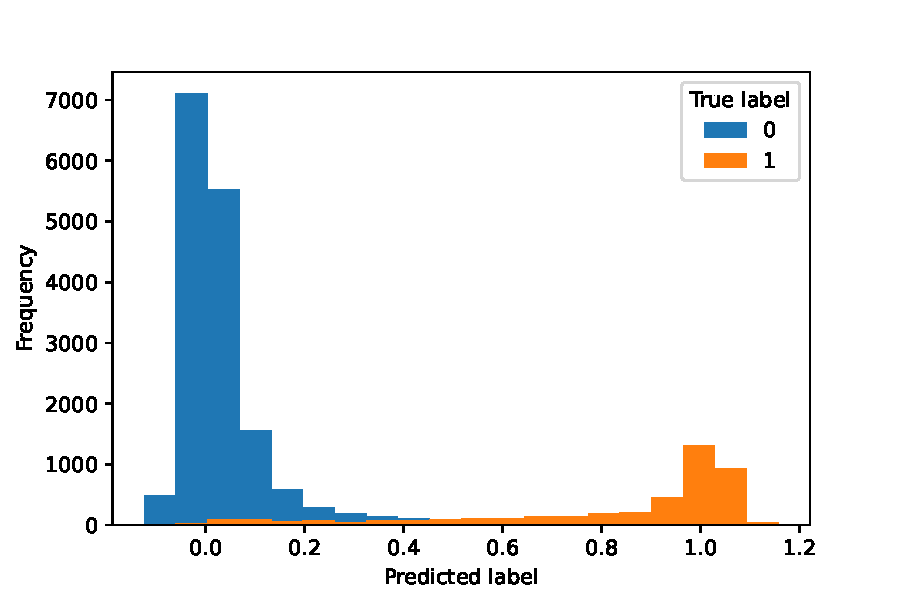
\includegraphics[width=\linewidth]{histogram-labels-bert-train.pdf}
        \subcaption{Predictions with \BertBase on the training set.}
        \label{subfig:bert_train}
    \end{subfigure}
    \hfill
    \begin{subfigure}{0.445\textwidth}
        \centering
        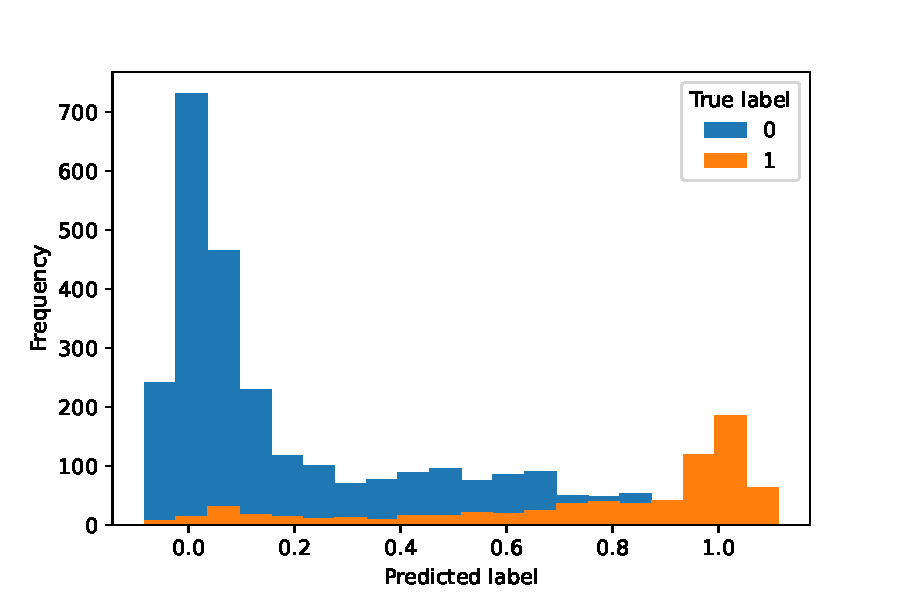
\includegraphics[width=\linewidth]{histogram-labels-bert-dev.pdf}
        \subcaption{Predictions with \BertBase on the validation set.}
        \label{subfig:bert_dev}
    \end{subfigure}
    \begin{subfigure}{0.445\textwidth}
        \centering
        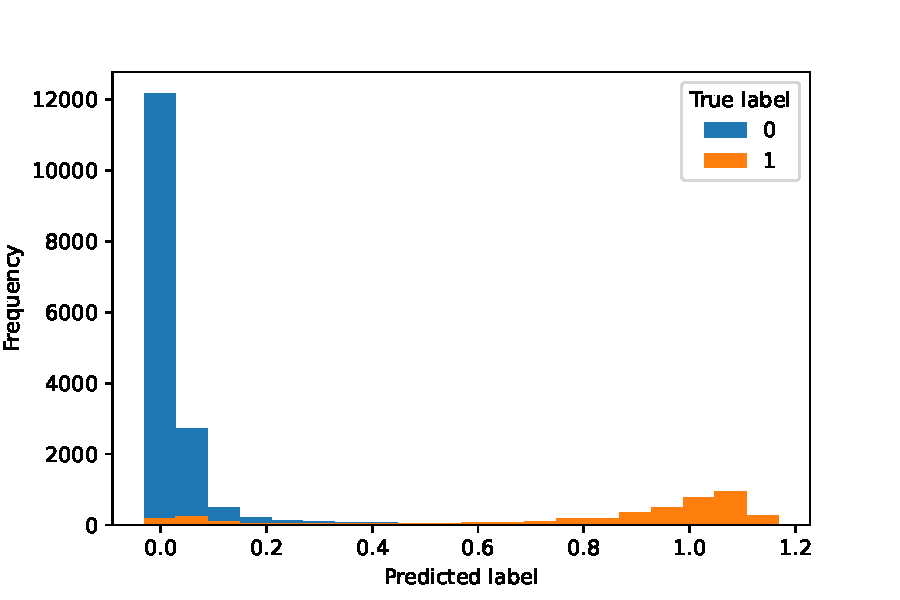
\includegraphics[width=\linewidth]{histogram-labels-roberta-train.pdf}
        \subcaption{Predictions with \RobertaBase on the training set.}
        \label{subfig:roberta_train}
    \end{subfigure}
    \hfill
    \begin{subfigure}{0.445\textwidth}
        \centering
        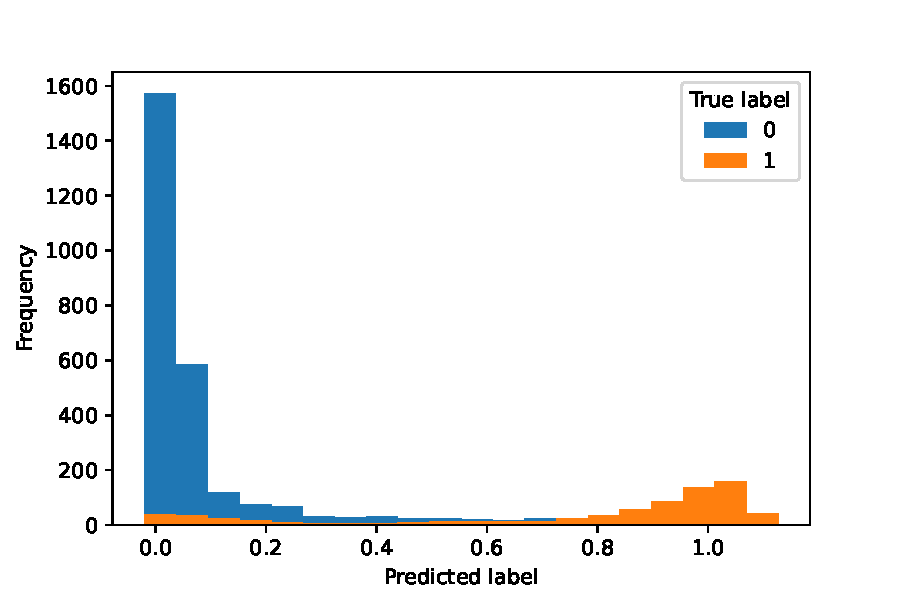
\includegraphics[width=\linewidth]{histogram-labels-roberta-dev.pdf}
        \subcaption{Predictions with \RobertaBase on the validation set.}
        \label{subfig:roberta_dev}
    \end{subfigure}
    \caption{Histograms of predicted labels on the training and validation sets for argument key point pairs with the \BertBase and \RobertaBase classifiers. For good classifiers, predicted labels should approximately equal the true label~(0~or~1).}
    \label{fig:frequency}
\end{figure*}
To find errors in the two trained matchers, \BertBase and \RobertaBase, in Figure~\ref{fig:frequency} we show histograms of predicted match scores with respect to ground-truth labels.
Both matchers classify most pairs correctly, which can be seen because the histogram spikes around~0 for the true no-match label and around~1 for the true match label.
We also observe that predictions on the training set are closer to the true label than on the development set for both \RobertaBase and \BertBase.
Even though we expect any machine-learned matcher to perform better on training data than on validation data, we see this as a room for improvement with better generalization.
We notice that in Figures~\ref{subfig:bert_train} and~\ref{subfig:roberta_train} both approaches predict non-matching argument key point pairs better than matching key points.
This effect is likely to occur because of the higher amount of non-matching pairs provided.
Most arguments match with only a few or even just a single key point.
But nonetheless each argument is compared to all other key points, hence the underlying data to learn from is imbalanced~\cite{BarandelaVSF2004}.
Though, experiments with using textual data augmentation to balance the dataset were unsuccessful.
Other approaches to balance the amount of matching and non-matching key points for each argument, e.g., oversampling or undersampling~\cite{Dietterich1995}, could resolve this issue.
We further identify, that for matching arguments and key points, predicted scores from \BertBase are spread a bit more than scores from \RobertaBase.

\begin{figure}
    \begin{tabularx}{\linewidth}{@{}lX@{}}
        Arg. & \textquote{School uniforms can be less comfortable than students' regular clothes.} \\
        KP & \textquote{School uniforms are expensive.} \\
        Pred. & \(0.48\) \\
    \end{tabularx}
    \caption{Argument and key point for the topic \textquote{We should abandon the use of school uniform} from the \ArgKP dataset~\cite{Bar-HaimEFKLS2020}.}
    \label{example-4-162-6}
\end{figure}
In Figures~\ref{subfig:bert_dev} and~\ref{subfig:roberta_dev}, we observe that the \BertBase matcher falsely classifies certain non-matching and matching pairs. The argument key point pair shown in Figure~\ref{example-4-162-6} seems to be particularily hard to classify.
One reason we identify is that this argument has no matching key points given in the training dataset.
Hence it is plausible that the \BertBase has not learned well how to classify matches for that type of argument, and therefore predicts a label of~\(0.48\).

\begin{figure}
    \begin{tabularx}{\linewidth}{@{}p{2em}X@{}}
        Arg. & \textquote{affirmative action can lead to people who are less qualified getting positions they would otherwise not be able to achieve} \\
        Arg. & \textquote{affirmative action discriminates the majority, preventing skilled workers from gaining employment over someone less qualified but considered to be a member of a protected minority group.}
    \end{tabularx}
    \caption{Matching arguments to the key point \textquote{Affirmative action reduces quality.} that are falsely classified as non-matching by the \BertBase matcher.}
    \label{example-5-110-113}
\end{figure}
\begin{figure}
    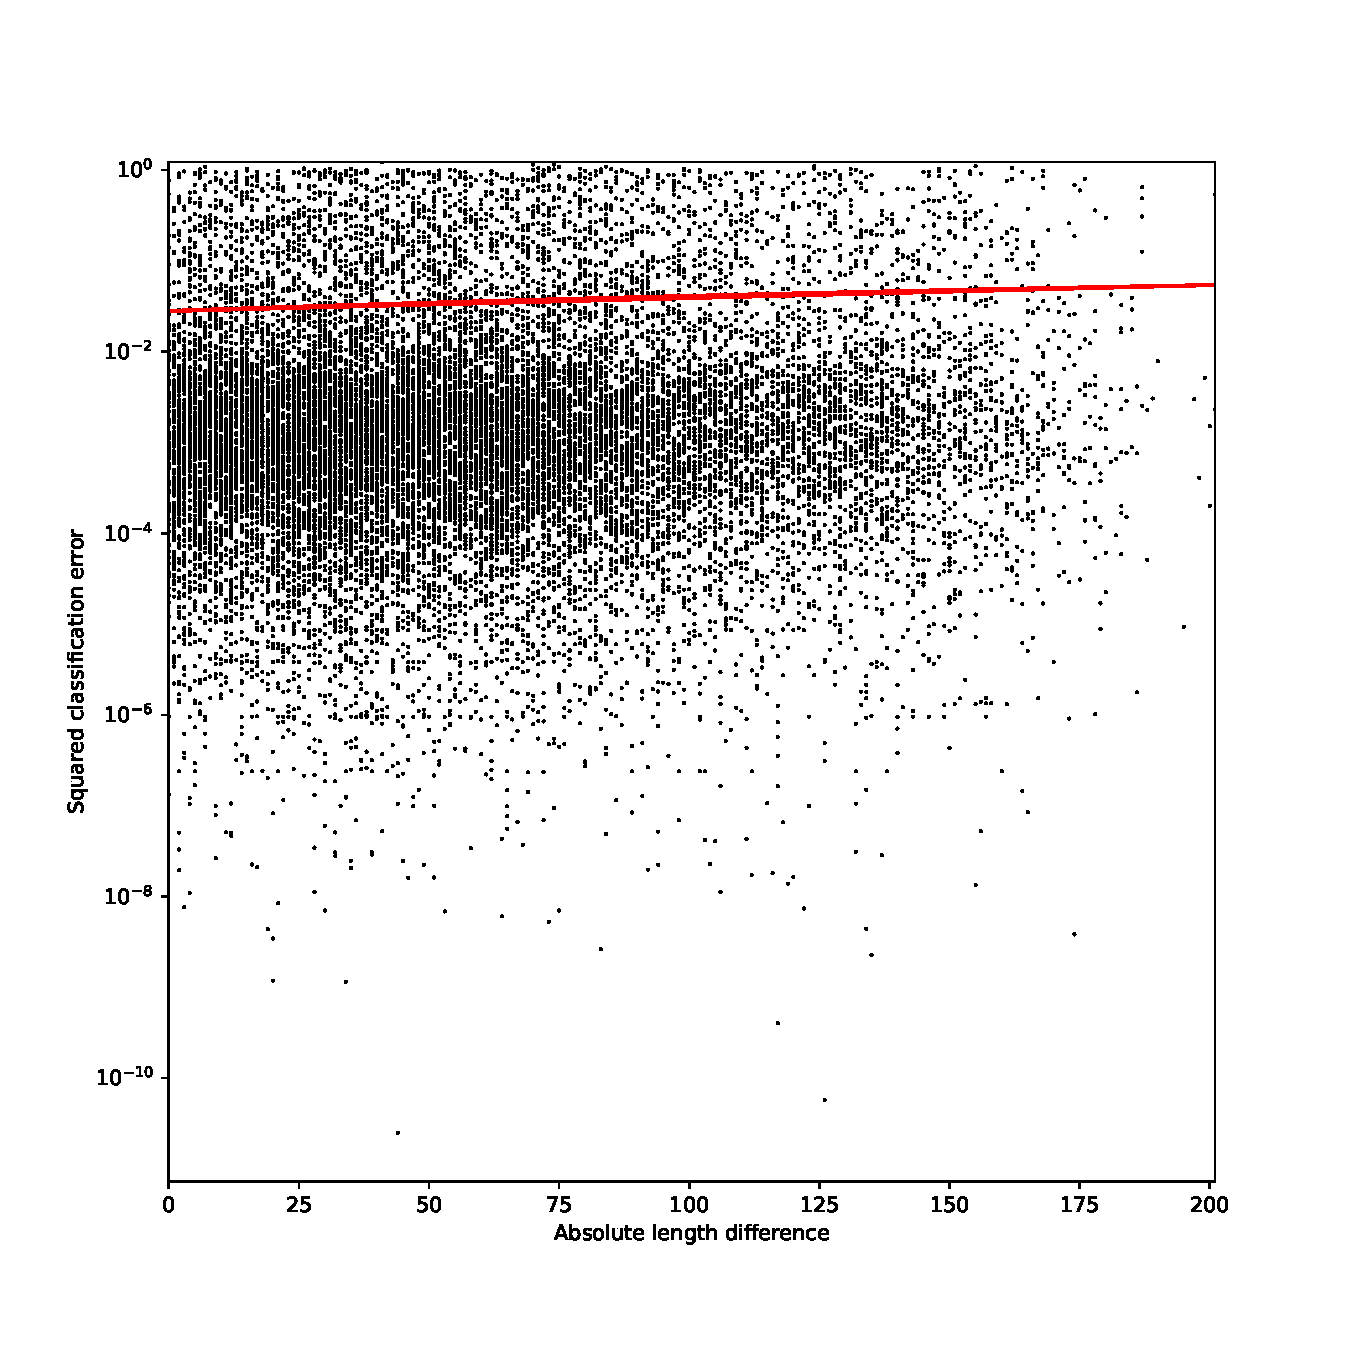
\includegraphics[width=\linewidth]{classification-error-length-difference-bert-train.pdf}
    \caption{Squared classification error and absolute length difference between each argument and key point pair from the validation set with the \BertBase matcher. The red line indicates the least squares polynomial fit.}
    \label{classification-error-length}
\end{figure}
The same \BertBase matcher falsely predicts some argument key point pairs as non-matching.
For example, it seems to be very difficult to predict matches for the key point \textquote{Affirmative action reduces quality.} from the topic \textquote{We should end affirmative action}, as shown in Figure~\ref{example-5-110-113}. These two arguments are longer than most arguments %\todo{from that topic?}
and especially longer than the key point.
It might be more challenging to reduce such longer arguments, containing more complex information, to very compact key points.
We confirm that observation by comparing the squared classification error with respect to the absolute difference between argument and key point lengths.
Figure~\ref{classification-error-length} shows a tendency of higher error with the \BertBase when the length difference between the argument and key point is large.
Comparable results can be observed for the \Roberta model.
We therefore identify length difference as a second general problem for both approaches.
